\documentclass{beamer}

% language
\usepackage[utf8]{inputenc}

\usepackage[procnames]{listings}
\usepackage{upquote}
\usepackage{color}
\usepackage{graphicx}
\usepackage{amsmath}
\usepackage{tikz}
\definecolor{bluekeywords}{rgb}{0.13,0.13,1}
\definecolor{greencomments}{rgb}{0,0.5,0}
\definecolor{redstrings}{rgb}{0.9,0,0}

%
\definecolor{LightCyan}{rgb}{0.60, 1, 1}
\definecolor{LightGreen}{rgb}{0.56, 0.93, 0.56}
\definecolor{LightGrey}{rgb}{0.83, 0.83, 0.83}
\definecolor{Amber}{rgb}{1.0, 0.75, 0.0}
\definecolor{DarkOrange}{rgb}{1.0, 0.55, 0.0}
\definecolor{DarkGreen}{rgb}{0.15, 0.85, 0.3}
%
\definecolor{deepblue}{rgb}{0,0,0.5}
\definecolor{deepred}{rgb}{0.6,0,0}
\definecolor{deepgreen}{rgb}{0,0.5,0}
%
\definecolor{darkmidnightblue}{rgb}{0.0, 0.2, 0.4}
%
\definecolor{keywords}{rgb}{0.54, 0.17, 0.89}
\definecolor{comments}{RGB}{0,0,113}
\definecolor{raed}{RGB}{160,0,0}
\definecolor{green}{RGB}{0,150,0}


\lstset{language=Python,
        breakatwhitespace=true,
        numberstyle=\tiny\color{gray},
        basicstyle=\ttfamily,
        keywordstyle=\color{keywords},
        commentstyle=\fontseries{lc}\selectfont\itshape\color{gray},
        stringstyle=\color{raed},
        showstringspaces=false,
        identifierstyle=\color{darkmidnightblue},
        procnamekeys={def,class}}

% -----
% Source and my dear thanks to:
% https://gist.github.com/eiriktsarpalis/6224587
%
\lstdefinelanguage{FSharp}%
{morekeywords={let, new, match, with, rec, open, module, namespace, type, of, member, %
and, for, while, true, false, in, do, begin, end, fun, function, return, yield, try, %
mutable, if, then, else, cloud, async, static, use, abstract, interface, inherit, finally },
  otherkeywords={ let!, return!, do!, yield!, use!, var, from, select, where, order, by },
  keywordstyle=\color{bluekeywords},
  sensitive=true,
  basicstyle=\ttfamily,
	breaklines=true,
  xleftmargin=\parindent,
	tabsize=4,
  morecomment=[l][\color{greencomments}]{///},
  morecomment=[l][\color{greencomments}]{//},
  morecomment=[s][\color{greencomments}]{{(*}{*)}},
  morestring=[b]",
  showstringspaces=false,
  literate={`}{\`}1,
  stringstyle=\color{redstrings},
}
% -----

\usepackage{listings}
\usepackage{adjustbox}
\newsavebox\listingboxname

% beamer theme
\usetheme{Boadilla}

% title page
\title[F\#]{Unser Pitch zur funktionalen Programmierung
}
\subtitle{mittels F\#}
\author[Parpart \& Thoma]{Christian Parpart \& Kei Thoma}
\institute[HU]{Humboldt Universität zu Berlin}
\date{27. Juni 2019}

% document
\begin{document}

\frame{\titlepage}

\begin{frame}
    \begin{center}
        {\Huge i = i + 1}
    \end{center}
\end{frame}

\begin{frame}
    \frametitle{Wir werden nicht:}
    \begin{enumerate}
        \item eine neue Programmiersprache lernen
        \item funktionale Programmieren lernen
    \end{enumerate}
\end{frame}

\frame{\titlepage}

\begin{frame}
    \frametitle{Inhalt}
    \tableofcontents
\end{frame}

\section{Nähe zur Mathematik}

\subsection{Immutability}

\begin{frame}[fragile]
    \frametitle{Immutability}
    \begin{minipage}[t]{0.5\linewidth}
        \begin{center}
            \textbf{Python}
        \end{center}
        \begin{lstlisting}[language=Python,numbersep=0pt,resetmargins=true]
a = 0

i = 1
i = i + 1
        \end{lstlisting}
        \end{minipage}%
        \begin{minipage}[t]{0.5\linewidth}
        \begin{center}
            \textbf{F\#}
        \end{center}
        \begin{lstlisting}[language=FSharp]
let a = 0

let mutable i = 1
i <- i + 1
        \end{lstlisting}
        \end{minipage}%
\end{frame}

\subsection{Notation}

\begin{frame}[fragile]
    \frametitle{Notation}
    \begin{minipage}[t]{0.5\linewidth}
        \begin{center}
            \textbf{Mathe}
        \end{center}
        \begin{align*}
a &= 1 \\
f: x &\mapsto x + a \\
\\
g&(f(x)) \\
(g& \circ f) (x) \\
        \end{align*}
    \end{minipage}%
    \begin{minipage}[t]{0.5\linewidth}
        \begin{center}
            \textbf{F\#}
        \end{center}
        \begin{lstlisting}[language=FSharp]
let a     = 1
let f (x) = x + a
            
g(f(x))
            
(g << f)(x)            
        \end{lstlisting}
\end{minipage}%
\end{frame}

\section{Seiteneffektfreiheit}

\begin{frame}[fragile]
    \frametitle{Seiteneffektfreiheit}
    \begin{minipage}[t]{0.4\linewidth}
        \begin{center}
            \textbf{Code}
        \end{center}
\begin{lstlisting}
let f(x) =
    let a = 2
    let b = 3
    a * b + x
\end{lstlisting}
    \end{minipage}%
    \begin{minipage}[t]{0.6\linewidth}
        \textbf{Eine Funktion, die nur von ihren Argumenten abhängt, ist seiteneffektfrei!} \\
        Wir gewinnen die folgenden Garantien:
    \begin{enumerate}
        \item Vorherbestimmtheit (Determinismus)
        \item Vereinfachte Code Verständlichkeit
        \item Vereinfachte Refaktorisierung
    \end{enumerate}
\end{minipage}%
\end{frame}

\section{Wiederverwendbarkeit}

\begin{frame}
    \frametitle{Wiederverwendbarkeit}
    \begin{columns}[c]
        \begin{column}{.7\textwidth}
            \begin{itemize}
                \item folgt aus der Seiteneffektfreiheit
                \item nicht aller Code ist 25 Zeilen lang
                \begin{itemize}
                    \item rechts im Bild: 1023 Zeilen
                    \item links im Bild: 15894 Zeilen: Seite zu klein ;-(
                \end{itemize}
            \end{itemize}
        \end{column}
        \begin{column}{.3\textwidth}
            \begin{center}
                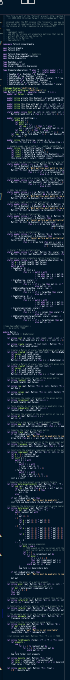
\includegraphics[scale=0.4]{long_code.png}
            \end{center}
        \end{column}
    \end{columns}
\end{frame}


\section{Verifizierbarkeit}

\begin{frame}
    \frametitle{Verifizierbarkeit}
    \begin{itemize}
        \item Theorem Proving und Mutable Variablen (Z3, CVC4)
        \item FP Programme sind leichter zu verifizieren
    \end{itemize}
\end{frame}

\begin{frame}
    \frametitle{Fazit}
    \begin{itemize}
        \item Probleme von Funktionaler Programmierung
        \begin{itemize}
            \item Schwierig sich rein zu denken
            \item Langsamer als C/C++ \\
            {\footnotesize(aber immer noch schneller als Python)}
            \item wenn es einmal läuft, wie ein Stein
        \end{itemize}
        \item Fun Fact: F\# steht für \_\_\_
    \end{itemize}
\end{frame}


\section{Fazit}

\begin{frame}
    \frametitle{Fazit}
    \begin{itemize}
        \item Probleme von Funktionaler Programmierung
        \begin{itemize}
            \item Schwierig sich rein zu denken
            \item Langsamer als C/C++ \\
            {\footnotesize(aber immer noch schneller als Python)}
            \item wenn es einmal läuft, wie ein Stein
        \end{itemize}
        \item Fun Fact: F\# steht für FUN
    \end{itemize}
\end{frame}

\section{Bonusmaterial}

\begin{frame}
    \frametitle{Bonusmaterial}
    \begin{center}
        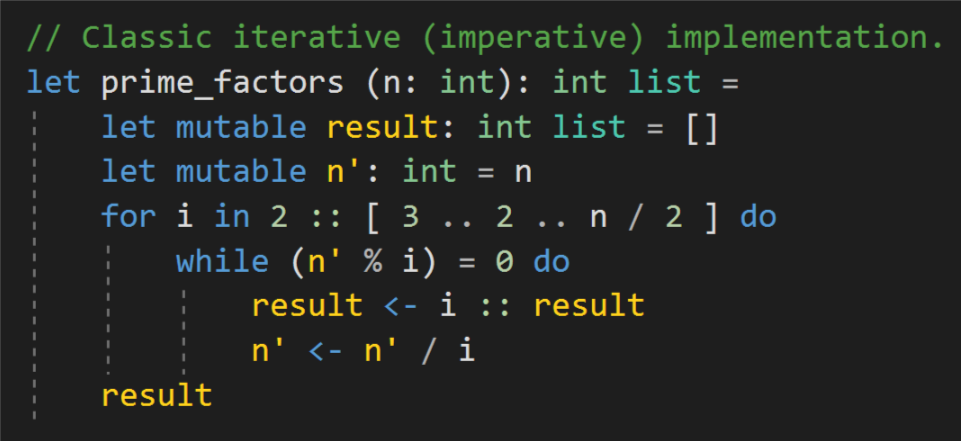
\includegraphics[scale=0.3]{naiv.png}
    \end{center}
\end{frame}

\begin{frame}
    \frametitle{Bonusmaterial}
    \begin{center}
            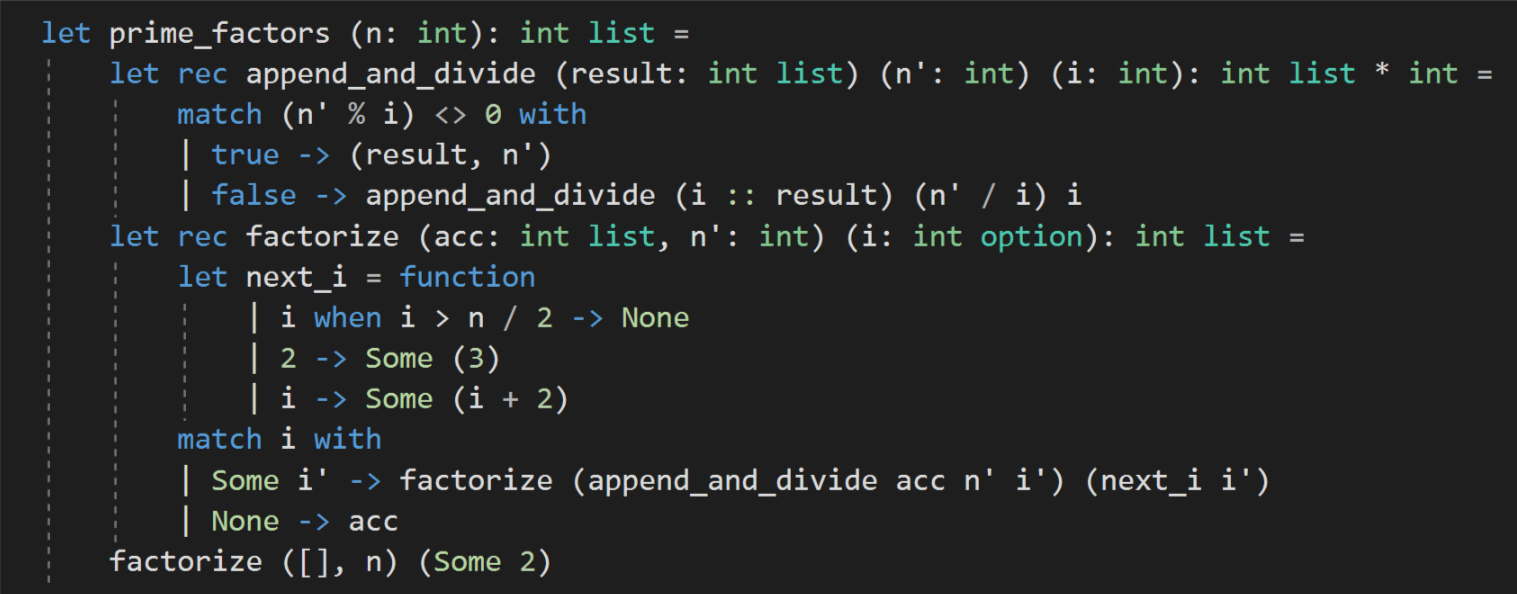
\includegraphics[scale=0.225]{primfaktorzerlegung_funktional.png}
    \end{center}
\end{frame}

\begin{frame}
    \frametitle{Bonusmaterial}
    \begin{center}
        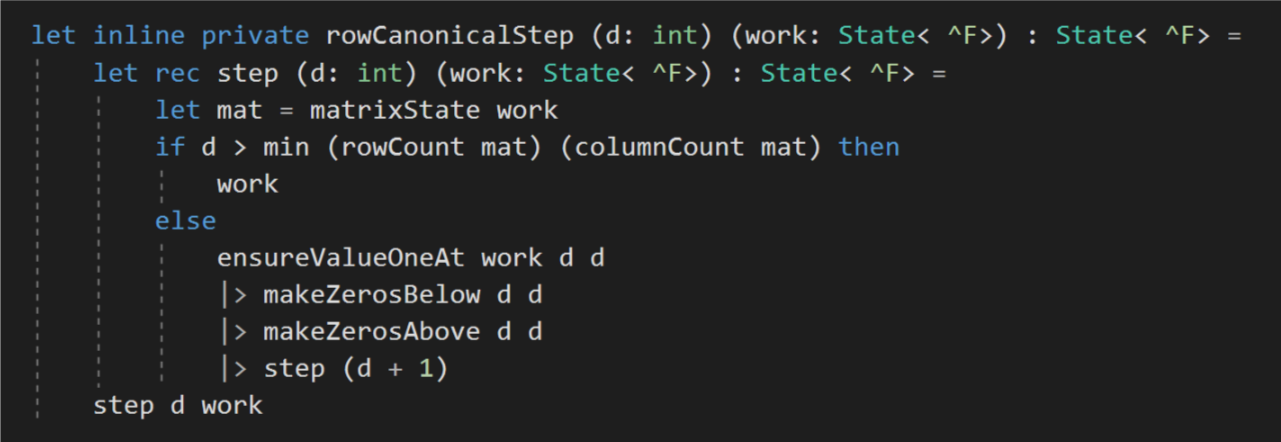
\includegraphics[scale=0.25]{funktionskomposition}
    \end{center}
\end{frame}



\end{document}
